%%% Local Variables:
%%% mode: latex
%%% TeX-master: "../doc"
%%% coding: utf-8
%%% End:
% !TEX TS-program = pdflatexmk
% !TEX encoding = UTF-8 Unicode
% !TEX root = ../doc.tex

This section describes the approaches and methods applied in the project. These consist of the general approach, the organisation methodology chosen, the use of Git version control and the project schedule set up at the beginning of the project.

\section{Realization of project}
The following subsections describe the realization of the project in detail.

\subsection{Proof that approach of bachelor thesis is applicable}
The first step as to realisation of this project was to prove whether the approach given by the bachelor thesis on which the project is founded is applicable. Since neither one of us has ever worked with Blazor or the related technologies used in the bachelor thesis, the consideration of the software prototype was of particular importance. Both the prototype (see chapter \ref{Prototype}) and the concept of mapping Toggl Track data to ATP data (see chapter \ref{Mapping concept}) have been investigated in detail. This was done using the documentation of the bachelor thesis, the software code of the prototype and the Blazor online documentation. Thus a fundamental understanding of the approach has been gained. Moreover, our .NET teacher, Mr. Rege, has agreed to provide technological support for Blazor and related technologies. In the light of all this, the approach has been considered applicable and therefore served as basis for the realisation of this project.

\subsection{Implementation of mapping concept}
To be able to actually handle data in the application, the mapping concept designed in the bachelor thesis (see chapter \ref{Mapping concept}) had to be implemented. The implementation generally follows the mapping concept apart from a few class attributes which were deleted since they were not considered to be needed.

\subsection{Graphical overview of difference between planning and tracking} \label{Charts}
Since the comparison between planned and tracked time should be displayed graphically, there had to be a possibility to display data using charts. The approach suggested in the bachelor thesis was to use the JavaScript library Charts.js and call it directly out of the application. However, this was not considered to be the best way to display charts since JavaScript code had to be added manually and called using code injection. Therefore, we decided to dedicate some time to investigate more elegant alternatives. The following packages offer functionality to create charts in Blazor without having to write JavaScript code:
\begin{itemize}
	\item Blazorise \cite{blazorise-url} - a multi-component library providing charts display functionality via an extension
	\item ChartsJs.Blazor \cite{chartsjs.blazor-url} - an open-source interface to the Charts.js JavaScript library
	\item Plotly.Blazor \cite{plotly-url} - an open-source charts display library available in multiple languages
	\item Radzen \cite{radzen-url} - a multi-component library
\end{itemize}
All four packages were tested by trying to include a sample chart into the application. Apart from ChartsJs.Blazor, which happened to have some installation issues, all packages could easily be installed and integrated. The following pictures show sample charts generated by the different packages being displayed in the ATP.

\begin{figure}[H]
	\centering
	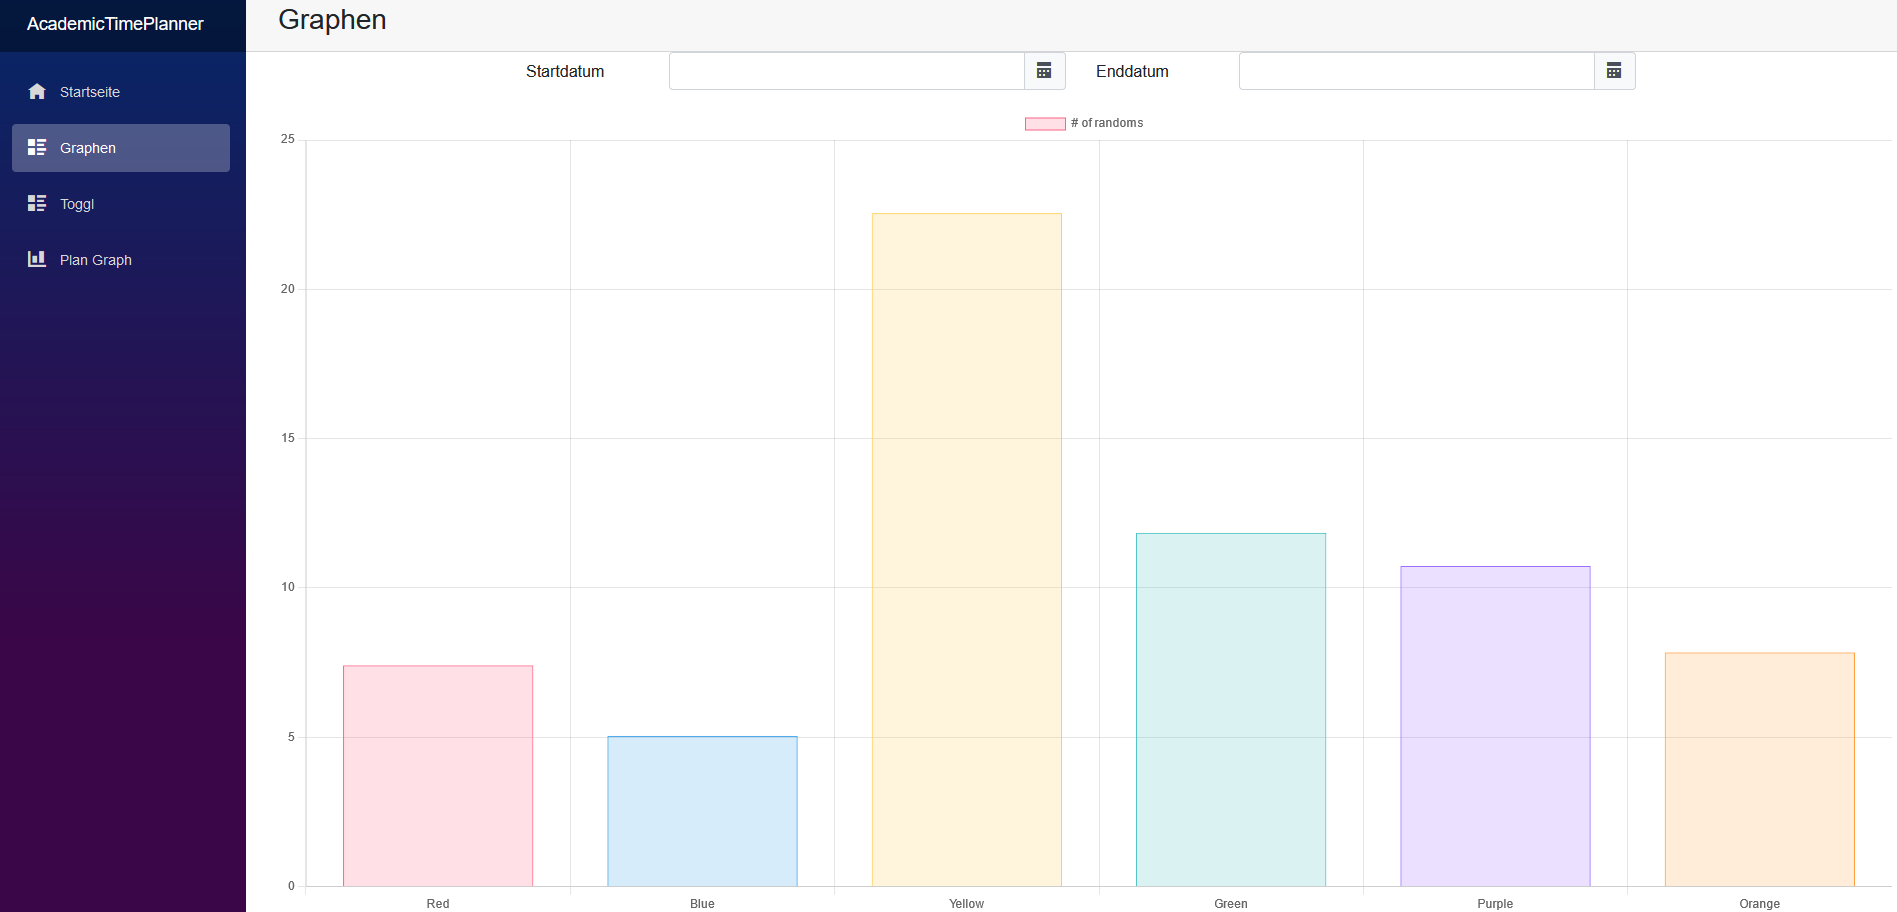
\includegraphics[width=1.0\columnwidth]{blazorise-charts}
	\caption{Blazorise sample charts on the ATP charts page}
	\label{figure5}
\end{figure}

\begin{figure}[H]
	\centering
	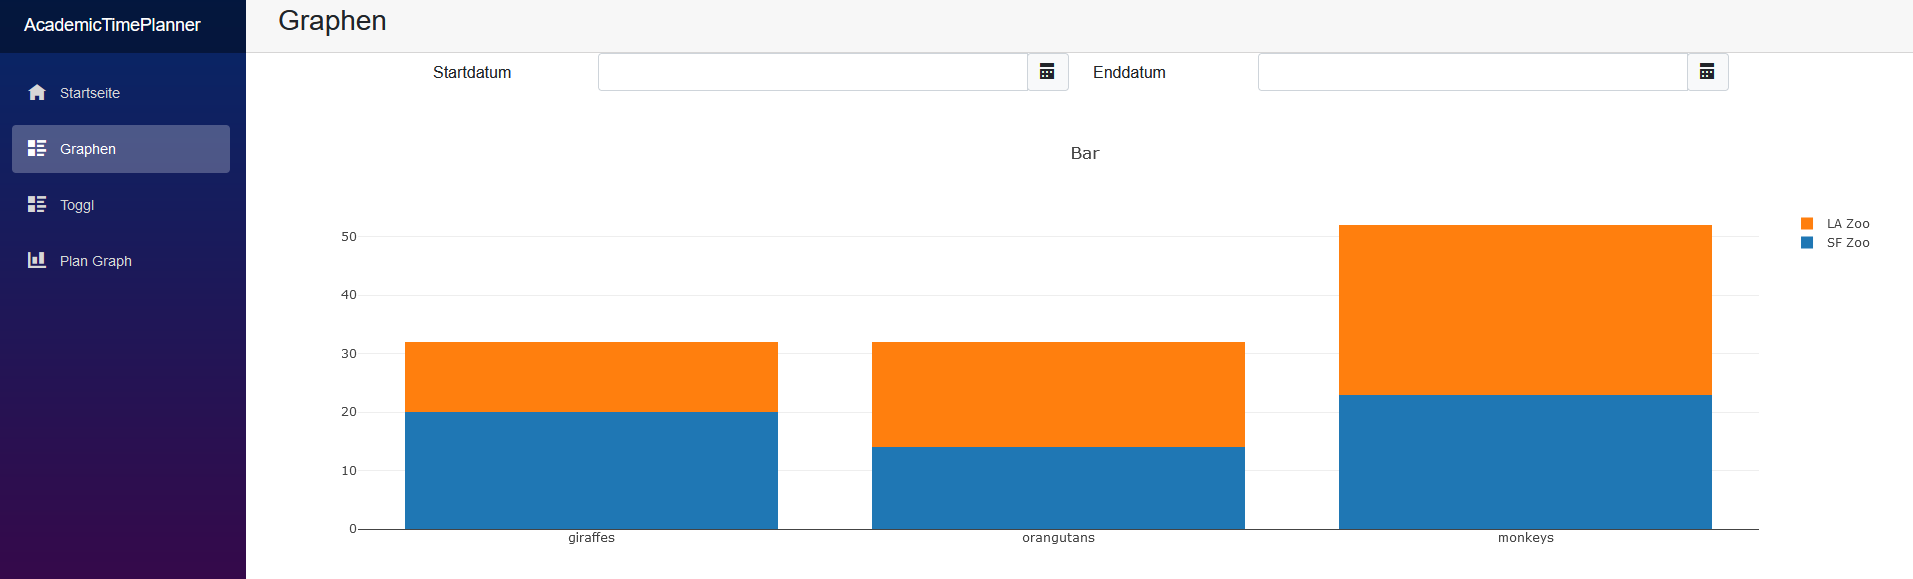
\includegraphics[width=1.0\columnwidth]{plotly-charts}
	\caption{Plotly.Blazor sample charts on the ATP charts page}
	\label{figure6}
\end{figure}

\begin{figure}[H]
	\centering
	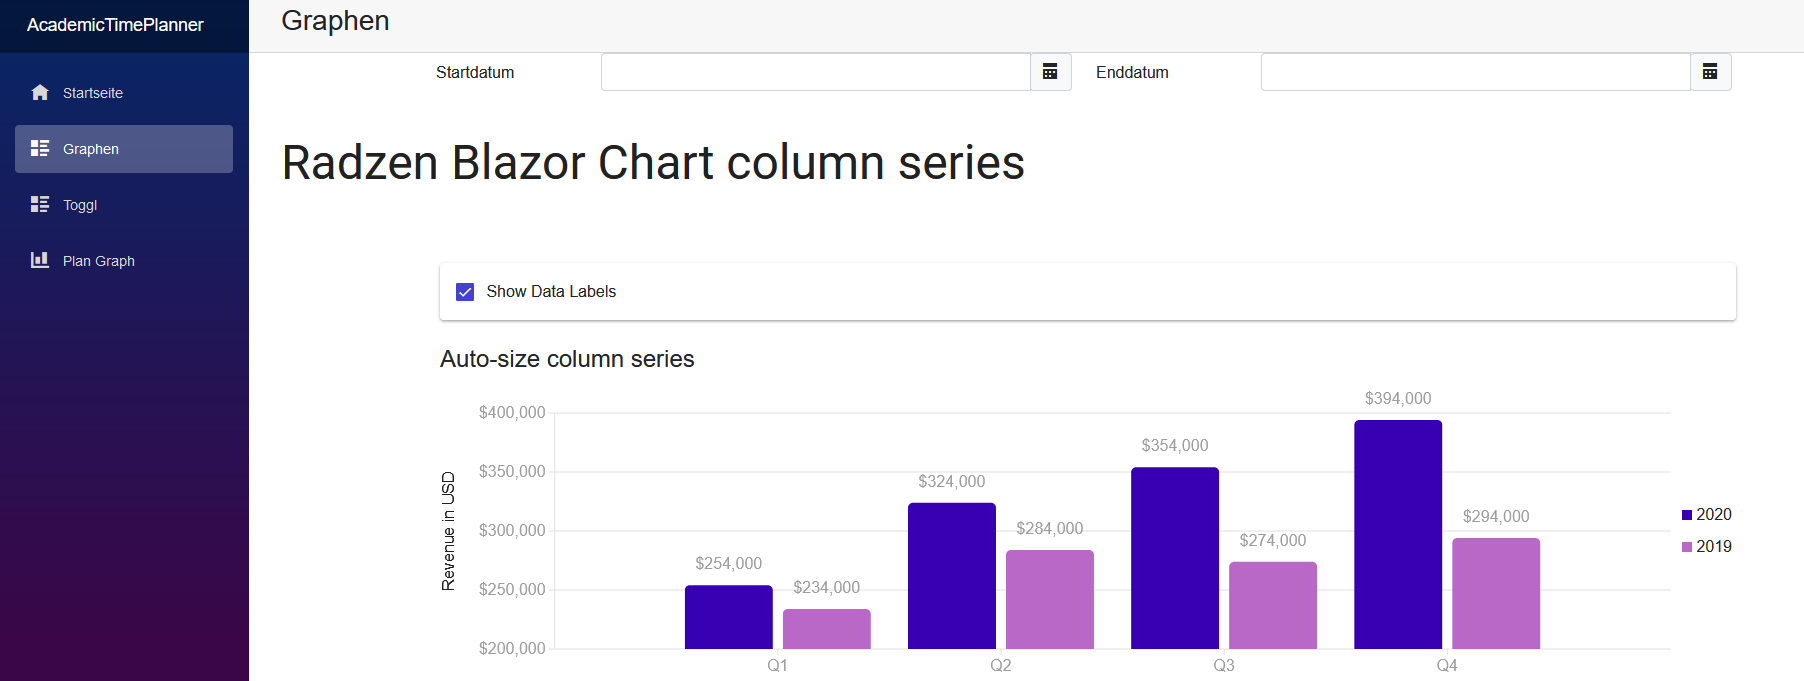
\includegraphics[width=1.0\columnwidth]{radzen-charts}
	\caption{Radzen sample charts on the ATP charts page}
	\label{figure7}
\end{figure}

For the realisation of the charts display, Plotly.Blazor was deemed to be the most suitable package for this application, since it focuses on exactly that functionality and is easier to use, compared to the other packages named above. The result of the implementation is described in more detail in chapter \ref{Graphical overview}

\subsection{Test projects}
To correctly simulate a working environment, test projects were created. To use a Toggl project in the application without actually having to fetch data from the Toggl API, a helper class providing a simulated Toggl project was created. A JSON file containing simulated planned data allowed for loading and using a plan project in the application. The combination of these two projects allowed the whole application to run without the need for real data while still displaying reasonable values for the user.

\subsection{Status display}
Following the project description, the next step was to add a status display as to when the ATP was last synchronized with Toggl Track, including a short overview of the loaded Toggl projects and their status and association with ATP plan projects. The results are described in chapter \ref{Status display}.

\subsection{Replacement of JavaScript code by C\# code} \label{JS replacement}
The technological prototype developed in the bachelor thesis included a few JavaScript (JS) code snippets used to display charts, provide a date picker and display a modal entry mask. From our point of view, the application should be implemented in C\# as far as possible, since JS code tends to be difficult for maintenance. Moreover, the integration of JavaScript into C\# code is slightly awkward. Therefore, it was decided to remove the JS snippets and to replace them by C\# code. As already mentioned in chapter \ref{Charts}, Plotly.Blazor was used instead of Charts.js. The modal entry mask and the date pickers were replaced by appropriate Blazor input components.

\subsection{Linking of planning and tracking data}
The final step, after planning data could be created, was to add functionality allowing for linking plan projects with Toggl projects. Since the Plan Projects pages already contained
numerous functionalities, a separate Blazor page was added for the linking. The results are described in chapter \ref{Linking}.

\section{Organization methodology}
For this project a reduced and modified version of SCRUM \cite{scrum_url} was chosen. The modifications include reducing the daily SCRUM meetings to two to three meetings a week, as we did not work on the project full time. One of these meetings was also attended by our project advisor Mr. Feisthammel. This meeting was usually held on Tuesday morning. There, a short progress report as well as the next weekly goals were discussed. Milestones as described in chapter \ref{Time management} have been defined. They roughly correspond with the two-week sprint plan. An additional reduction is the absence of a sprint review as we do something similar in the weekly meetings described above. The point system as well as the burn down chart were also dropped.

\section{Git}
For appropriate software code management, the Git version control system and the online service GitHub (see chapter \ref{Version control}) have been used. The software code was stored in a GitHub repository named "academic-time-planner". The main branch always represented the current state of the software, containing all tested and approved features. New features were implemented via feature branches named according to the pattern "feature/name-of-member/feature-description". The software tests were executed automatically via GitHub Actions (see chapter \ref{GitHub Actions}) on every push to a feature branch. The result of the automated tests were taken into account in the feature pull requests. The documentation was kept in the same repository and was treated like the software code in the sense that additions and changes had to be reviewed and approved via pull requests, as was the software code. Documentation branches were named after the "documentation/name-of-member/section-description". Tasks were managed via GitHub issues (see chapter \ref{GitHub Issues}).

\section{Time management} \label{Time management}
Four milestones were proposed at the beginning of the project. They were taken from the project outline and include three programming milestones and one documentation milestone. The first one was the implementation of the overview of difference between plan and tracking, followed by the application status display. The final programming milestone was composed of the import and export as well as the creation of plan projects. After this the documentation had to be finalized. These milestones were meant as a guideline to see if the progress was adequate or if we had to rethink our approach. Those milestones were created and managed in GitHub (see chapter \ref{GitHub}). 

\section{Pair programming}
Pair programming \cite{pairprogramming-url} is a form of programming in which one person is writing code while the other person can focus on keeping an overview. The second person is also in charge of helping finding solutions or researching something needed for the next step while the first types the agreed upon solution. The pair should regularly alternate with who is typing and who is not, to keep it balanced. This programming approach is preferable with new and/or unknown technology as well as with complex code as the problems and challenges can be discussed together. Moreover, the likelihood of making mistakes together is smaller, since both programmers are looking at the code. For this reasons pair programming was heavily used in the second sprint, as unknown technology was used, and the implementation of loading and displaying data was fairly complex at first. 

\section{Unit tests}
To ensure that the methods function as intended, unit tests are necessary. They are also needed to check if everything still works after refactoring. To this end, unit tests were written for every backend class where it was deemed necessary. This includes the mapping classes described in the chapter \ref{Mapping concept} as well as the classes DataManager and JSONHandler. These classes are essential for the whole application to work correctly, as a mistake in them would affect all the other classes. Most of these tests check if the handling of JSON files and the projects that are generated with them work as intended. The test cases are listed in the following table.
\\ \\
\begin{tabular}{||c|c|p{8cm}||}
	\cline{1-3}
	Class & Method & Case \\
	\hline \hline
	JSONHandler & saveJson & Are a plan project and all its components written correctly in the JSON file. \\
	\hline
	 & loadJson & Is the JSON file correctly parsed to a functioning plan project. \\
	\hline
	DataManager & Constructor & Are the lists for plan projects and Toggl projects empty as expected. \\ 
	\hline
	& UpdateTogglData & Is an empty Toggl project list correctly updated. \\
	\hline
	&  & Is a non empty Toggl project list correctly updated. \\
	\hline
	&  & Is a Toggl project that is deleted on TogglTrack, but still exists in the application, moved to the correct list.\\
	\hline
	& & Is a Toggl entry that got reassigned to a different Toggl project not duplicated.\\
	\hline
	& GetChartData & Are empty plan project and Toggl project lists returned empty as expected.\\
	\hline
	& & Are non empty plan project and Toggl project lists returned correctly.\\
	\hline
	& GetTogglLoadOverview & Is an empty list returned correctly.\\
	\hline
	& & Is the overview correctly returned when the Toggl project has an associated plan project.\\
	\hline
	& & Is the overview correctly returned when the Toggl project has no associated plan project. \\
	\hline
	& & Is a Toggl project that is deleted on TogglTrack, but still exists in the application, displayed correctly. \\
	\hline
	& \scriptsize{UpdateTogglDictionaryInPlanProjects} & Are the percentages in the plan project updated correctly.\\
	\hline
	TogglService & GetTogglProjects & Are the Toggl projects returned as expected.\\
	\hline
	& & Can a Toggl project be handled if there is no task.\\
	\hline
	& & Is a Toggl project with a Toggl task handled correctly.\\
	\hline
	& & Is the sum of durations of a Toggl project without any entries returned as 0 as expected.\\
	\hline
	& & Is the sum of the duration of entries without a project returned the correctly. \\
	\cline{1-3}
\end{tabular}